\chapter{Arhitektura i dizajn sustava}
		
		\textbf{\textit{dio 1. revizije}}\\

		\textit{ Potrebno je opisati stil arhitekture te identificirati: podsustave, preslikavanje na radnu platformu, spremišta podataka, mrežne protokole, globalni upravljački tok i sklopovsko-programske zahtjeve. Po točkama razraditi i popratiti odgovarajućim skicama:}
	\begin{itemize}
		\item 	\textit{izbor arhitekture temeljem principa oblikovanja pokazanih na predavanjima (objasniti zašto ste baš odabrali takvu arhitekturu)}
		\item 	\textit{organizaciju sustava s najviše razine apstrakcije (npr. klijent-poslužitelj, baza podataka, datotečni sustav, grafičko sučelje)}
		\item 	\textit{organizaciju aplikacije (npr. slojevi frontend i backend, MVC arhitektura) }		
	\end{itemize}
	
	Arhitektura našeg sustava temeljit će se na kombinaciji modernih tehnologija kako bismo ostvarili funkcionalan i skalabilan sustav. Sustav će se podijeliti na tri ključna podsustava: 
	\begin{itemize}
		\item 	\textit{\textbf{Web poslužitelj}}		
		\item 	\textit{\textbf{Web preglednik}}	
		\item 	\textit{\textbf{Baza podataka}}
	\end{itemize}
	Organizacija će biti usklađena s MVC (Model-View-Controller) konceptom, omogućavajući neovisnost između različitih dijelova sustava te olakšavajući razvoj, ispitivanje i dodavanje novih funkcionalnosti.
	
	\textit{Web preglednik}, kao program koji omogućuje korisnicima pregled web-stranica i multimedijalnih sadržaja, igra ključnu ulogu. Klijenti, putem web preglednika, šalju zahtjeve web poslužitelju kako bi pristupili željenim resursima.
	
	\textit{Web poslužitelj} je osnova rada web aplikacije i odgovoran je za komunikaciju između klijenta i aplikacije. Komunikacija se odvija putem HTTP protokola, koji omogućuje prijenos informacija na webu. Poslužitelj pokreće web aplikaciju i prosljeđuje joj zahtjeve koje prima od klijenata.	

	\textit{\textbf{Web aplikacija}}, smještena na poslužitelju, obrađuje zahtjeve korisnika. Ovisno o tim zahtjevima, pristupa poslužitelju baze podataka i na temelju dobivenih podataka, putem web poslužitelja, šalje odgovor korisnicima. Aplikacija se sastoji od backend i frontend dijela, koji se razvijaju koristeći različite tehnologije u skladu s opisanom arhitekturom sustava. Konkretno, za backend dio koristit ćemo Spring, dok će za frontend biti korišten React, što je u skladu s MVC načelima.
		
	Ključna karakteristika MVC koncepta je nezavisan razvoj pojedinih dijelova aplikacije. Ova karakteristika rezultira jednostavnijim ispitivanjem, kao i olakšanim razvojem i dodavanjem novih svojstava u sustav.
	
	MVC koncept sastoji se od tri osnovna dijela:
	
	\begin{itemize}
		\item 	\textit{\textbf{Model:}}	središnja komponenta sustava koja predstavlja dinamičke strukture podataka neovisne o korisničkom sučelju. Model upravlja podacima, logikom i pravilima aplikacije, primajući ulazne podatke od Controllera
		\item 	\textit{\textbf{View:}}	odgovara za prikaz podataka, poput grafičkih elemenata. Moguć je različiti prikaz istih informacija, kao što su grafički ili tablični prikazi podataka
		\item 	\textit{\textbf{Controller:}} primarno prima ulazne podatke od korisnika i prilagođava ih za daljnju interakciju s Modelom ili Viewom. Kontrolira korisničke zahtjeve i izvodi daljnju interakciju s ostalim elementima sustava
	\end{itemize}
	
	Ovaj pristup omogućuje jasnu organizaciju sustava i olakšava daljnji razvoj i održavanje.

		

				
		\section{Baza podataka}
			
			
		Kao sustav za upravljanje bazama podataka za našu aplikaciju odabrali smo PostgreSQL. To je otvoren sustav za upravljanje bazama koji omogućuje pohranu, upravljanje i analizu podataka.
			
		Sama baza podataka sadržavat će šest tablica. One će služiti za pohranu podataka o korisnicima te njihovom korištenju aplikacije. Korištenje će se spremati u obliku događaja koje stvaraju ili posjećuju te recenzija koje pišu za određene događaje. Isto tako spremat će se sama zainteresiranost za događaje te notifikacije koje posjetitelji žele primati za događaje s određenim karakteristikama.
			
		Sami odabir PostgreSQL-a je u njegovoj pouzdanosti, skalabilnosti i podrške za napredne SQL funkcionalnosti, što će nam omogućiti lakše te učinkovitije upravljanje podacima.
			Baza podataka ove aplikacije sastoji se od sljedećih entiteta: 
			\begin{itemize}
			\item 	Korisnik
			\item 	Organizator	
			\item 	Događaj
			\item 	Recenzija
			\item 	Zainteresiranost
			\item 	Notifikacija
		\end{itemize}
		
		
			\subsection{Opis tablica}
			

				\textbf{Korisnik} -  ovaj entitet sadržava sve važne informacije o korisniku aplikacije. Sadrži atribute: korisnik\_id koji je automatski dodijeljen, username, lozinka, email i uloga u aplikaciji. Ovaj entitet u vezi je Many-to-One s entitetom organizator preko atributa organizator\_id.
				
				
				\begin{longtblr}[
					label=none,
					entry=none
					]{
						width = \textwidth,
						colspec={|X[7,l]|X[6, l]|X[20, l]|}, 
						rowhead = 1,
					} %definicija širine tablice, širine stupaca, poravnanje i broja redaka naslova tablice
					\hline \SetCell[c=3]{c}{\textbf{korisnik}}	 \\ \hline[3pt]
					\SetCell{LightGreen}korisnik\_id & INT	&  	Primarni ključ tablice, dodjeljuje se automatski  	\\ \hline
					username	& VARCHAR & Jedinstveno ime koje korisnik odabire tijekom registracije  	\\ \hline 
					lozinka & VARCHAR & Lozinka koju korisnik odabire tijekom registracije  \\ \hline 
					email & VARCHAR	&  Jedinstveni email korisnika		\\ \hline 
					uloga & SMALL INT/INT &  Uloga koju korisnik ima unutar aplikacije(admin, posjetitelj, organizator)		\\ \hline 
				\end{longtblr}
				
							\textbf{Organizator } -  Ovaj entitet sadržava informacije o organizatoru događaja. Sadrži atribute: organizator\_id, naziv\_organizacije, adresa, poveznica, clanarina. Ovaj entitet u vezi je One-to-Many s entitetom dogadaj preko atributa organizator\_id.
			
			
			\begin{longtblr}[
				label=none,
				entry=none
				]{
					width = \textwidth,
					colspec={|X[9,l]|X[6, l]|X[20, l]|}, 
					rowhead = 1,
				} %definicija širine tablice, širine stupaca, poravnanje i broja redaka naslova tablice
				\hline \SetCell[c=3]{c}{\textbf{organizator}}	 \\ \hline[3pt]
				\SetCell{LightGreen}organizator\_id & INT	&  	Primarni ključ tablice, ujedno i strani ključ iz tablice korisnik 	\\ \hline
				naziv\_organizacije	& VARCHAR & Naziv organizacije kojoj pripada organizator  	\\ \hline 
				adresa & VARCHAR & Adresa organizacije  \\ \hline 
				poveznica & VARCHAR	&  Poveznica na web stranicu organizacije		\\ \hline 
				clanarina & BOOLEAN &  Plaćena članarina		\\ \hline 
			\end{longtblr}
			
							\textbf{Dogadaj } -  ovaj entitet sadržava informacije o događaju. Sadrži atribute: dogadaj\_id, organizator\_id, naziv\_dogadaja, vrsta, lokacija, trajanje, vrijeme\_pocetka, cijena\_ulaznice, opis, galerija. Ovaj entitet u vezi je Many-to-One s entitetom Organizator preko atributa organizator\_id te u vezi One-to-Many s entitetom recenzija preko atributa dogadaj\_id.
			
			
			\begin{longtblr}[
				label=none,
				entry=none
				]{
					width = \textwidth,
					colspec={|X[7,l]|X[6, l]|X[20, l]|}, 
					rowhead = 1,
				} %definicija širine tablice, širine stupaca, poravnanje i broja redaka naslova tablice
				\hline \SetCell[c=3]{c}{\textbf{dogadaj}}	 \\ \hline[3pt]
				\SetCell{LightGreen}dogadaj\_id & INT	&  	Primarni ključ tablice, dodjeljuje se automatski  	\\ \hline				\SetCell{LightBlue} organizator\_id	& INT & Strani ključ iz tablice organizator koji se odnosi na njegov ID  	\\ \hline 
				naziv\_dogadaja	& VARCHAR & Naziv događaja  	\\ \hline 
				vrsta & VARCHAR & Vrsta događaja(koncert, kazališna predstava ...)  \\ \hline 
				lokacija & VARCHAR	&  Lokacija događaja		\\ \hline 
				opis\_lokacije & VARCHAR & Kratki opis lokacije, adresa, kat …	\\ \hline 
				trajanje & INTERVAL & Trajanje događaja u danima \\ \hline 
				vrijeme\_pocetka & TIMESTAMP & Datum i vrijeme početka događaja \\ \hline 
				cijena\_ulaznice & NUMERIC & Cijena ulaznice na događaj \\ \hline 
				opis & VARCHAR & Kratki opis samog događaja \\ \hline 
				galerija & VARCHAR & Link do web stranice gdje se nalaze video snimke ili fotografije \\ \hline  
			\end{longtblr}
			
							\textbf{Recenzija} -  ovaj entitet sadržava informacije o recenziji događaja. Sadrži atribute: recenzija\_id, posjetitelj\_id, događaj\_id, tekst, ocjena. Ovaj entitet u vezi je Many-to-One s entitetom korisnik preko atributa posjetitelj\_id te u vezi Many-to-One s entitetom dogadaj preko atributa dogadaj\_id.
			
			
			\begin{longtblr}[
				label=none,
				entry=none
				]{
					width = \textwidth,
					colspec={|X[7,l]|X[6, l]|X[20, l]|}, 
					rowhead = 1,
				} %definicija širine tablice, širine stupaca, poravnanje i broja redaka naslova tablice
				\hline \SetCell[c=3]{c}{\textbf{recenzija}}	 \\ \hline[3pt]
				\SetCell{LightGreen}recenzija\_id & INT	&  	Primarni ključ tablice, dodjeljuje se automatski  	\\ \hline
				\SetCell{LightBlue}posjetitelj\_id	& INT & Strani ključ iz tablice korisnik koji se odnosi na njegov ID	\\ \hline 
				\SetCell{LightBlue}dogadaj\_id & INT & Strani ključ iz tablice dogadaj koji se odnosi na njegov ID \\ \hline 
				tekst & VARCHAR	&  Kratki tekst recenzije	\\ \hline 
				ocjena & SMALL INT/INT & Ocjena od 1-10, opcionalna	\\ \hline 
			\end{longtblr}
			
							\textbf{Zainteresiranost} -  ovaj entitet sadržava informacije o zainteresiranosti posjetitelja za određeni događaj. Sadrži atribute: zainteresiranost\_id, posjetitelj\_id, dogadaj\_id, kategorija, obavijesti. Ovaj entitet u vezi je Many-to-One s entitetom korisnik preko atributa posjetitelj\_id te u vezi Many-to-One s entitetom dogadaj preko atributa dogadaj\_id.
			
			
			\begin{longtblr}[
				label=none,
				entry=none
				]{
					width = \textwidth,
					colspec={|X[9,l]|X[6, l]|X[20, l]|}, 
					rowhead = 1,
				} %definicija širine tablice, širine stupaca, poravnanje i broja redaka naslova tablice
								\hline \SetCell[c=3]{c}{\textbf{zainteresiranost}}	 \\ \hline[3pt]
				\SetCell{LightGreen}zainteresiranost\_id & INT	&  	Primarni ključ tablice, dodjeljuje se automatski  	\\ \hline
				\SetCell{LightBlue}posjetitelj\_id	& INT & Strani ključ iz tablice korisnik koji se odnosi na njegov ID	\\ \hline 
				\SetCell{LightBlue}dogadaj\_id & INT & Strani ključ iz tablice dogadaj koji se odnosi na njegov ID \\ \hline 
				kategorija & SMALL INT/INT	&  Jedna od tri kategorije: Sigurno dolazim, možda dolazim ili ne dolazim	\\ \hline 
				obavijesti & BOOLEAN & Želi li posjetitelj biti obaviješten o promjeni na događaju	\\ \hline 
			\end{longtblr}
			
							\textbf{Notifikacija } -  ovaj entitet sadržava informacije o notifikacijama koje će posjetitelji primati vezano uz tražene događaje filtirane po vrsti ili lokaciji. Sadrži atribute: notifikacija\_id, posjetitelj\_id, vrsta, lokacija. Ovaj entitet u vezi je Many-to-One s entitetom korisnik preko atributa posjetitelj\_id te u vezi Many-to-One s entitetom dogadaj preko atributa vrsta i lokacija.
			
			
			\begin{longtblr}[
				label=none,
				entry=none
				]{
					width = \textwidth,
					colspec={|X[7,l]|X[6, l]|X[20, l]|}, 
					rowhead = 1,
				} %definicija širine tablice, širine stupaca, poravnanje i broja redaka naslova tablice
				\hline \SetCell[c=3]{c}{\textbf{notifikacija}}	 \\ \hline[3pt]
				\SetCell{LightGreen}notifikacija\_id & INT	&  	Primarni ključ tablice, dodjeljuje se automatski  	\\ \hline
				\SetCell{LightBlue}posjetitelj\_id	& INT & Strani ključ iz tablice korisnik koji se odnosi na njegov ID \\ \hline
				vrsta & VARCHAR & Vrsta događaja za koji posjetitelj želi primiti obavijest o njegovu stvaranju, opcionalno\\ \hline 
				lokacija & VARCHAR	&  Lokacija događaja za koji posjetitelj želi primiti obavijest o njegovu stvaranju, opcionalno		\\ \hline 
			\end{longtblr}
			
							
			
			\subsection{Dijagram baze podataka}
				U ovom potpoglavlju potrebno je umetnuti dijagram baze podataka. Primarni i strani ključevi moraju biti označeni, a tablice povezane. Bazu podataka je potrebno normalizirati. Podsjetite se kolegija "Baze podataka".
				
				\begin{figure}
					\centering
					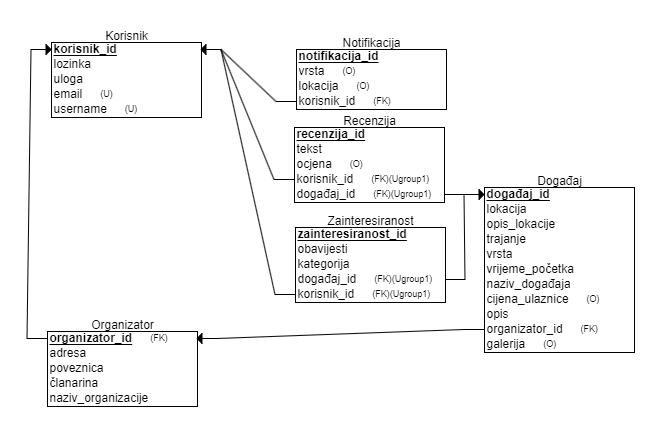
\includegraphics[scale=0.7]{slike/baza.PNG}
					\caption{Dijagram baze podataka}
				\end{figure}
			\eject
			
			
		\section{Dijagram razreda}
		
			Na slikama \textbf{4.2, 4.3, 4.4 i 4.5} su prikazani razredi koji pripadaju \textit{backend} dijelu projekta. 
			\newline
			\newline
			Razredi prikazani na slici \textbf{4.2} su razredi kontroleri. Ti razredi su ključni dijelovi koji upravljaju pristiglim zahtjevima, određuju rute te obrađuju logiku aplikacije. Obično se koriste za implementaciju HTTP metoda poput \textbf{GET, POST, PUT i DELETE} za obrađivanje zahtjeva koji dolaze od klijenata. Razredi koji imaju svoje kontrolere su \textbf{Korisnik, Organizator, Admin, Posjetitelj, Događaj, Notifikacija, Recenzija i Zainteresiranost}.
			\newline
			
			\textbf{KorisnikController} ima metode: 
			\begin{itemize}
				\item getAll - vraća listu Korisnika
				\item getKorisnikById - ako postoji Korisnik sa tim id, njega vraća
				\item getCurrentUser - kao argument prima Korisnika, a vraća KorisnikDTO
				\item register - kao argument prima KorsnikDTO, a vraća ResponseEntity koji je string
			\end{itemize}
			
			Isto ima i člansku varijablu tipa KorisnikService preko koje se obavlja poslovna logika (operacije nad podacima, pristupanje bazi podataka ili komunikacija s vanjskim servisima).
			\newline
			
				\textbf{OrganizatorController} ima metode: 
			\begin{itemize}
				\item getDetails - kao argument prima Korisnika, a vraća OrganizatorDTO
				\item register - kao argument prima OrganizatorDTO, a vraća ResponseEntity koji je string
			\end{itemize}
			
			Isto ima i članske varijable tipa KorisnikService i OrganizatorService preko koje se obavlja poslovna logika (operacije nad podacima, pristupanje bazi podataka ili komunikacija s vanjskim servisima).
			\newline
			\newline
			Razredi prikazani na slici \textbf{4.3} su razredi servisi. Razredi servisi u Spring Bootu predstavljaju komponente koje sadrže poslovnu logiku aplikacije, pristupaju podacima i obavljaju operacije koje nisu specifične za obradu HTTP zahtjeva. Oni često služe kao posrednici između kontrolera i sloja pristupa podacima (Repository sloj) te obavljaju ključne funkcije za obradu podataka, poslovnu logiku i vanjske integracije.
			Razredi koji imaju svoje servise su \textbf{Korisnik, Organizator, Admin, Posjetitelj, Događaj, Notifikacija, Recenzija i Zainteresiranost}.
			\newline
			
			\textbf{KorisnikService} ima metode: 
			\begin{itemize}
				\item listAll - vraća listu Korisnika
				\item findById - prima id kao argument, a ako postoji Korisnik s tim id, njega vraća
				\item findByUsername - prima username kao argument, a ako postoji korisnik s tim usernamom njega vraća
				\item findByEmail - prima email kao argument, a ako postoji korisnik s tim emailom njega vraća
				\item registerUser - kao argument prima KorsnikDTO, a boolean ovisno o uspješnosti
			\end{itemize}
			
			Isto ima i člansku varijablu tipa KorisnikRepository. Razred repozitorija u Spring Bootu predstavlja sloj pristupa podacima (data access layer) i obično se koristi za komunikaciju s bazom podataka. Ovi repozitoriji pružaju apstrakciju za operacije nad podacima, kao što su dohvaćanje, spremanje, ažuriranje ili brisanje podataka.
			\newline
			
			\textbf{OrganizatorService} ima metode: 
			\begin{itemize}
				\item findById - prima id kao argument, a ako postoji Organizator sa tim id, njega vraća
				\item registerOrganizator - kao argument prima OrganizatorDTO, a vraća boolean ovisno o uspješnosti
			\end{itemize}
			
			Razredi prikazani na slici 4.5. su razredi modeli. Struktura baze podataka u aplikaciji odražava se upravo model razredima; osim što imaju svoje pripadne atributa, razredi također implementiraju metode koje ostvaruju interakciju s bazom podataka. \\ 
			\\ Razred Korisnik reprezentira općeg korisnika aplikacije. Specificira ga atribut "uloga" koja određuje je li korisnik administrator, posjetitelj ili organizator.
			\\ Razred Organizator reprezentira korisnika s organizatorskim računom. Organizatori mogu pregledavati svoje postojeće događaje i postavljati nove događaje.
			\\ Razred Recenzija reprezentira korisnikov osvrt na događaj u obliku ocjene i komentara.
			\\ Razred Notifikacija reprezentira obavijest koja se šalje korisniku. Korisnik ima mogućnost uključiti notifikacije za određenu vrstu događaja te za lokaciju na kojoj se događaji organiziraju.
			\\ Razred Zainteresiranost reprezentira korisnikovu interakciju s postavljenim događajima. Korisnikova zainteresiranost ima tri razine: "sigurno dolazim", "možda dolazim", "ne dolazim".
			\\ Razred Dogadaj reprezentira događaj koji je postavio organizator. Lokacija događaja predstavljena je gradskom četvrti - kvartom.
			
			\pagebreak
			
			\begin{figure}[H]
				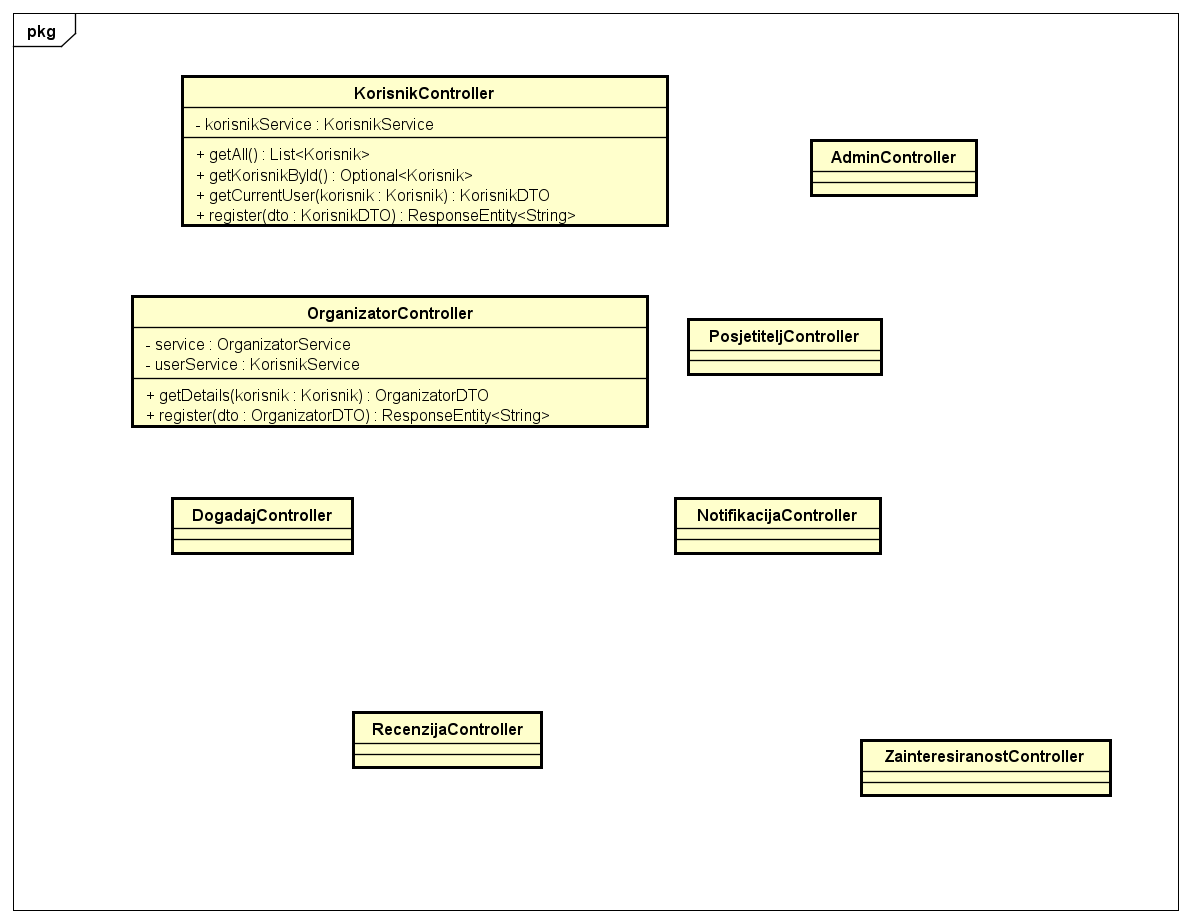
\includegraphics[scale=0.5]{dijagramiKlasa/Dijagram razreda - Kontroleri.png} %veličina slike u odnosu na originalnu datoteku i pozicija slike
				\centering
				\caption{Dijagram razreda - Kontroleri}
				\label{fig:promjene}
			\end{figure}
			
			\begin{figure}[H]
				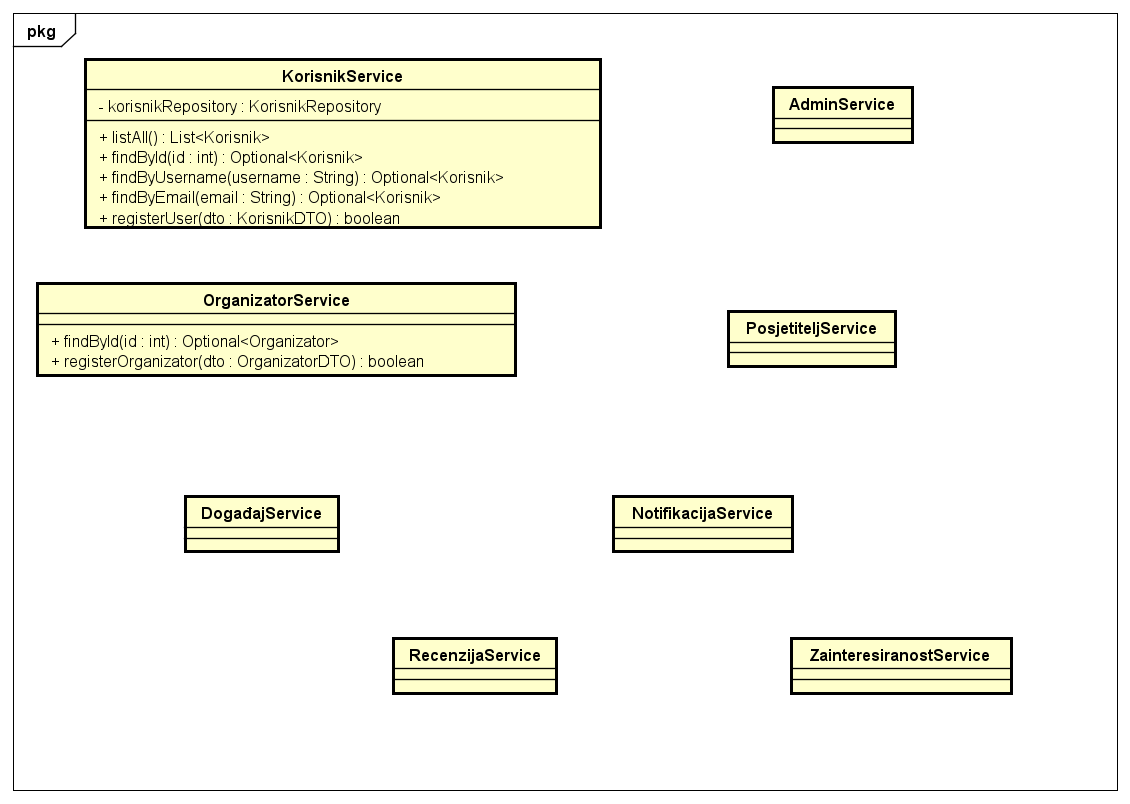
\includegraphics[scale=0.5]{dijagramiKlasa/Dijagram razreda - Servisi.png} %veličina slike u odnosu na originalnu datoteku i pozicija slike
				\centering
				\caption{Dijagram razreda - Servisi}
				\label{fig:promjene}
			\end{figure}
			
			\begin{figure}[H]
				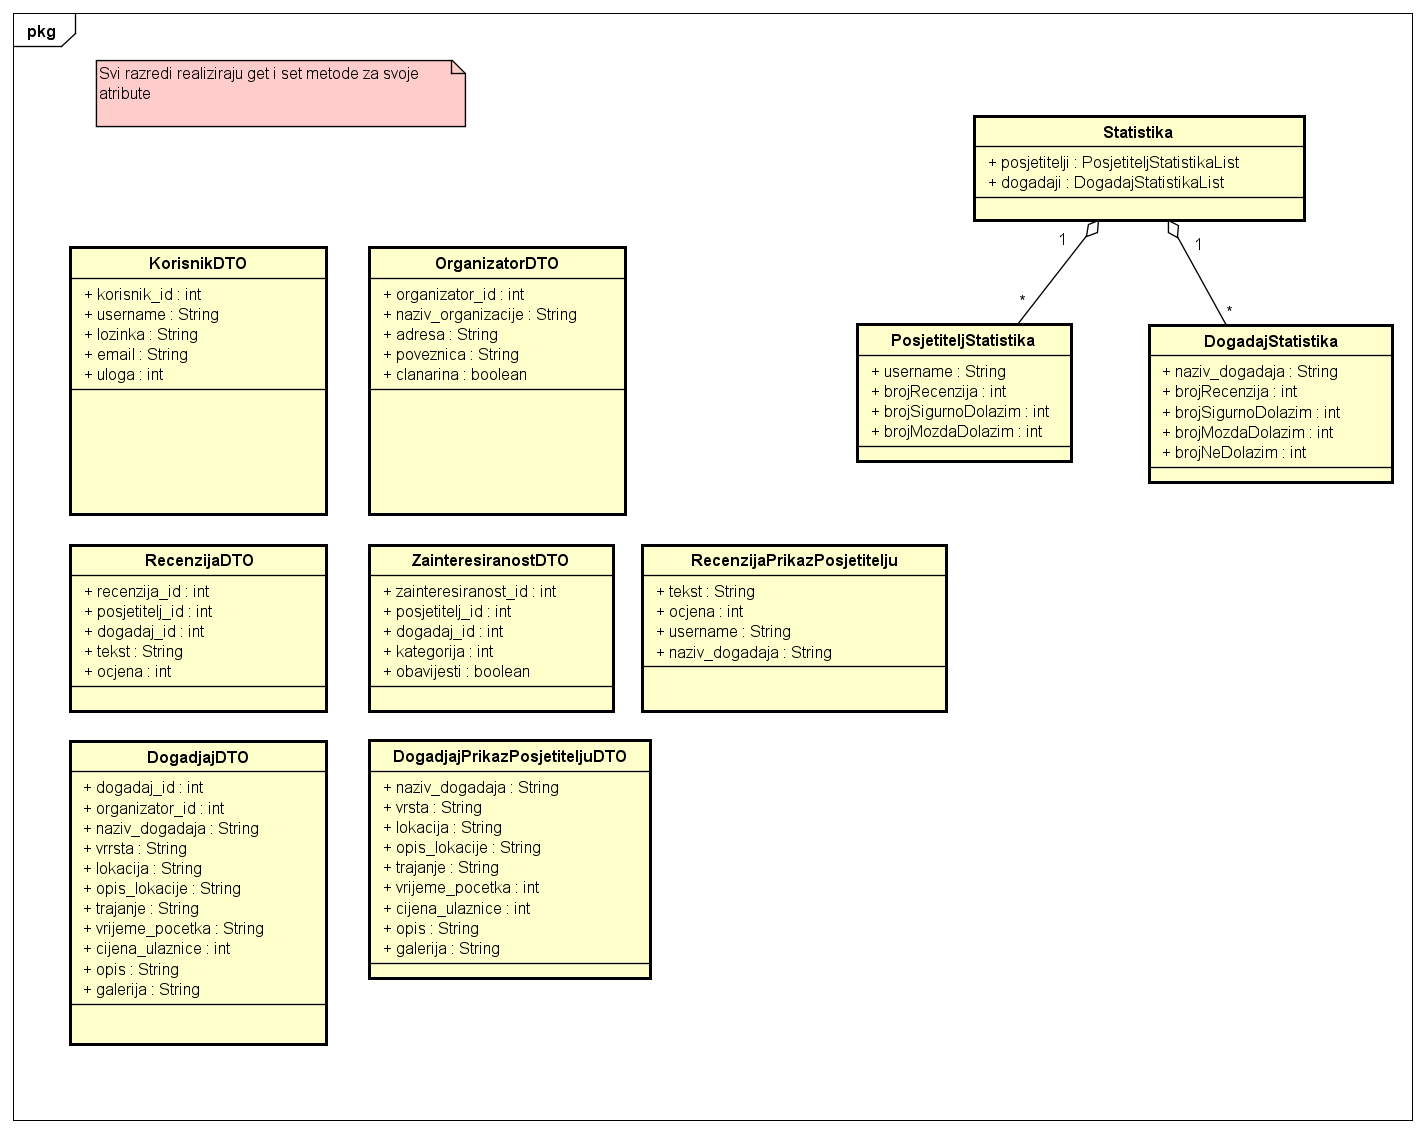
\includegraphics[scale=0.4]{dijagramiKlasa/Dijagram razreda - DTO.png} %veličina slike u odnosu na originalnu datoteku i pozicija slike
				\centering
				\caption{Dijagram razreda - Data Transfer Objects}
				\label{fig:promjene}
			\end{figure}
			
			
			\begin{figure}[H]
				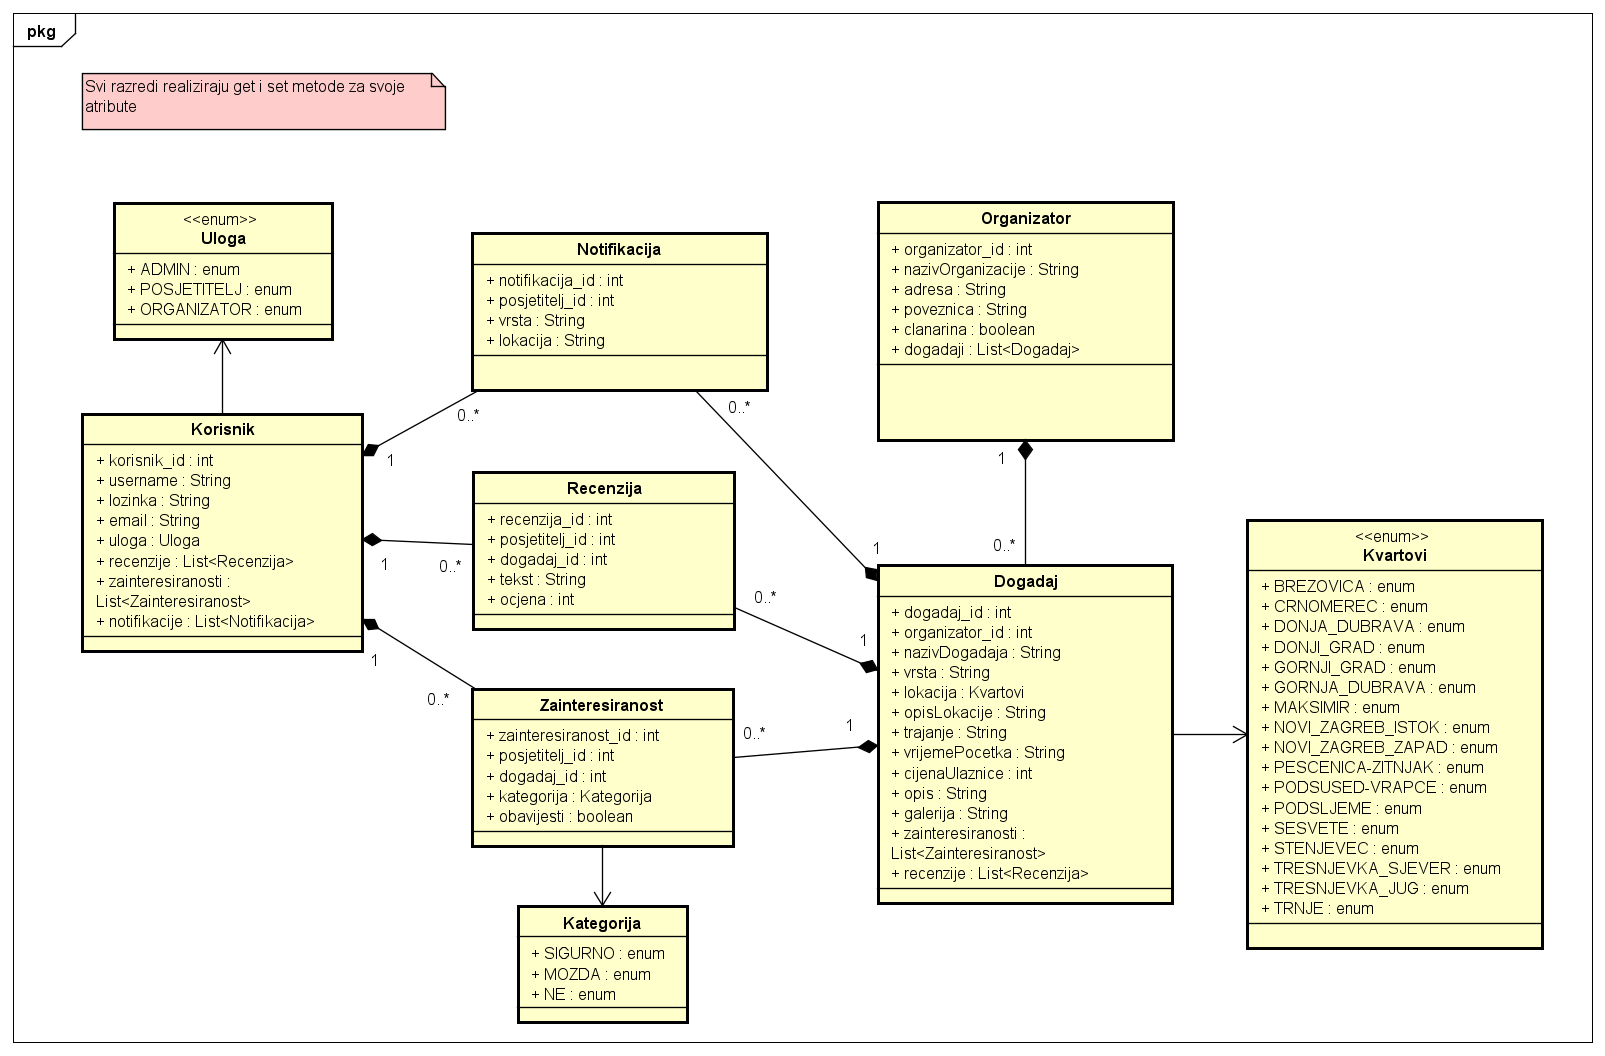
\includegraphics[scale=0.4]{dijagramiKlasa/Dijagram razreda - Models v5.png} %veličina slike u odnosu na originalnu datoteku i pozicija slike
				\centering
				\caption{Dijagram razreda - Models}
				\label{fig:promjene}
			\end{figure}
			
			\textbf{\textit{dio 2. revizije}}\\			
			
			\textit{Prilikom druge predaje projekta dijagram razreda i opisi moraju odgovarati stvarnom stanju implementacije}
			
			
			
			\eject
		
		\section{Dijagram stanja}
			
			
			\textbf{\textit{dio 2. revizije}}\\
			
			\textit{Potrebno je priložiti dijagram stanja i opisati ga. Dovoljan je jedan dijagram stanja koji prikazuje \textbf{značajan dio funkcionalnosti} sustava. Na primjer, stanja korisničkog sučelja i tijek korištenja neke ključne funkcionalnosti jesu značajan dio sustava, a registracija i prijava nisu. }
			
			
			\eject 
		
		\section{Dijagram aktivnosti}
			
			\textbf{\textit{dio 2. revizije}}\\
			
			 \textit{Potrebno je priložiti dijagram aktivnosti s pripadajućim opisom. Dijagram aktivnosti treba prikazivati značajan dio sustava.}
			
			\eject
		\section{Dijagram komponenti}
		
			\textbf{\textit{dio 2. revizije}}\\
		
			 \textit{Potrebno je priložiti dijagram komponenti s pripadajućim opisom. Dijagram komponenti treba prikazivati strukturu cijele aplikacije.}